% Appendix X

\chapter{Further LO QCD fit of kaon multiplicities}\label{app:Fit}

%----------------------------------------------------------------------------------------

A similar fit than the one perfomed in Chapter~\ref{ch:FF} was done with COMPASS data on isoscalar target. The result of the fit is presented in Fig.~\ref{pic:FApp} and the parameters in Table~\ref{tab:ParApp}.

\begin{table}[!h]
  \begin{center}
    \begin{tabular}{ | c | c c c c c | }
      \hline
      \hline
       & N & $\alpha$ & $\beta$ & $\gamma$ & $\delta$ \\
      \hline
      \hline
      $\D{K}{fav}$ & 0.05148 $\pm$ 0.0003 & -1.4 $\pm$ 0.1 & 0.18 $\pm$ 0.05 & -1.8 $\pm$ 0.4 & 3.6 $\pm$ 0.1 \\
      $\D{K}{s}$ & 0.024 $\pm$ 0.001 & 19 $\pm$ 5 & 25 $\pm$ 2 & - & -  \\
      $\D{K}{unf}$ & 0.0081 $\pm$ 0.0002 & 2.8 $\pm$ 0.5 & 12 $\pm$ 1 & - & - \\
      $\D{K}{glu}$ & 0.086 $\pm$ 0.006 & 30 $\pm$ 4 & 13 $\pm$ 5 & - & - \\
      \hline
      \hline
    \end{tabular}
  \end{center}
  \caption{Fit parameters for $Q^2_0$ = 1 (GeV/$c$)$^2$. The associated $\chi^2$ is of 3.2.}
  \label{tab:ParApp}
\end{table}


\begin{figure}[!h]
  \centering
	\subfloat[$zD^{K}_{fav}$]{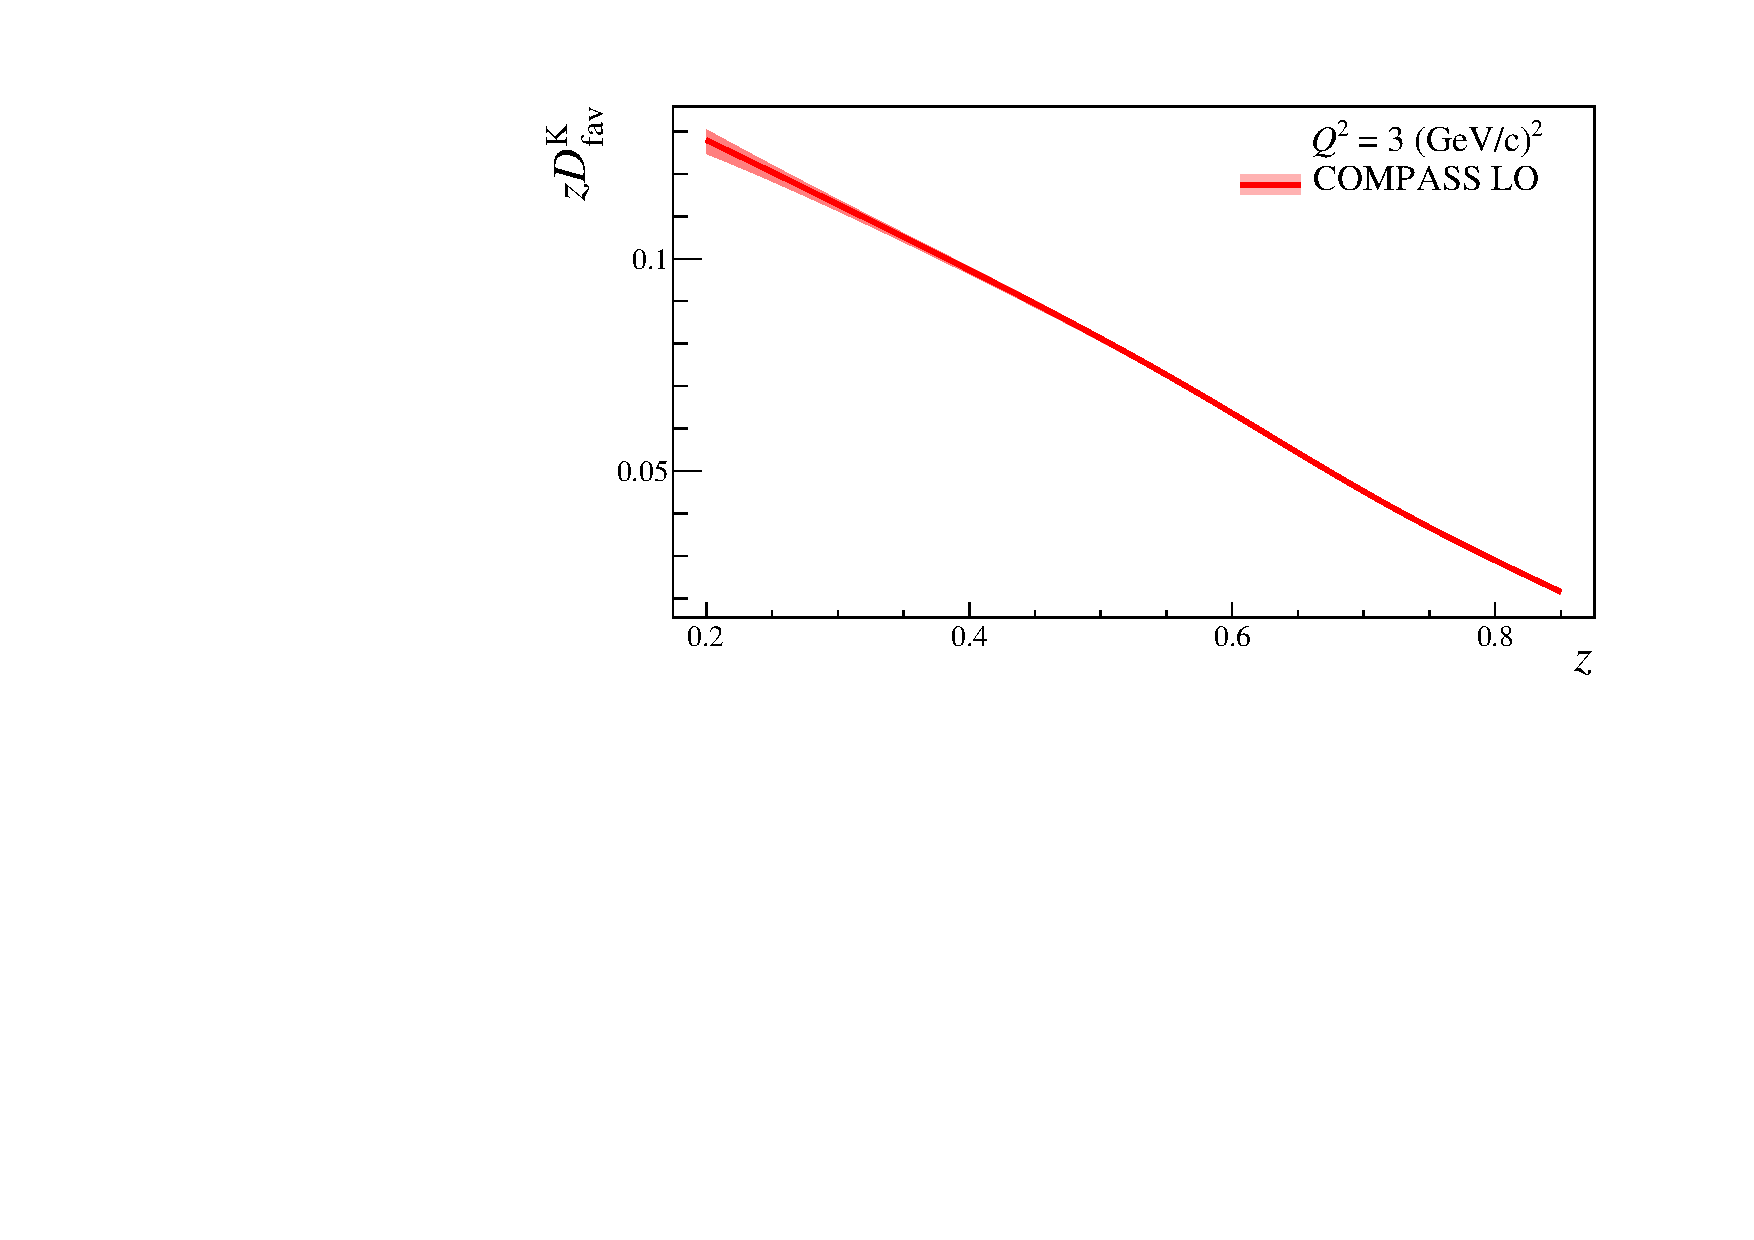
\includegraphics[scale=0.4]{./gfx/dfav.pdf}}
  \subfloat[$zD^{K}_{unf}$]{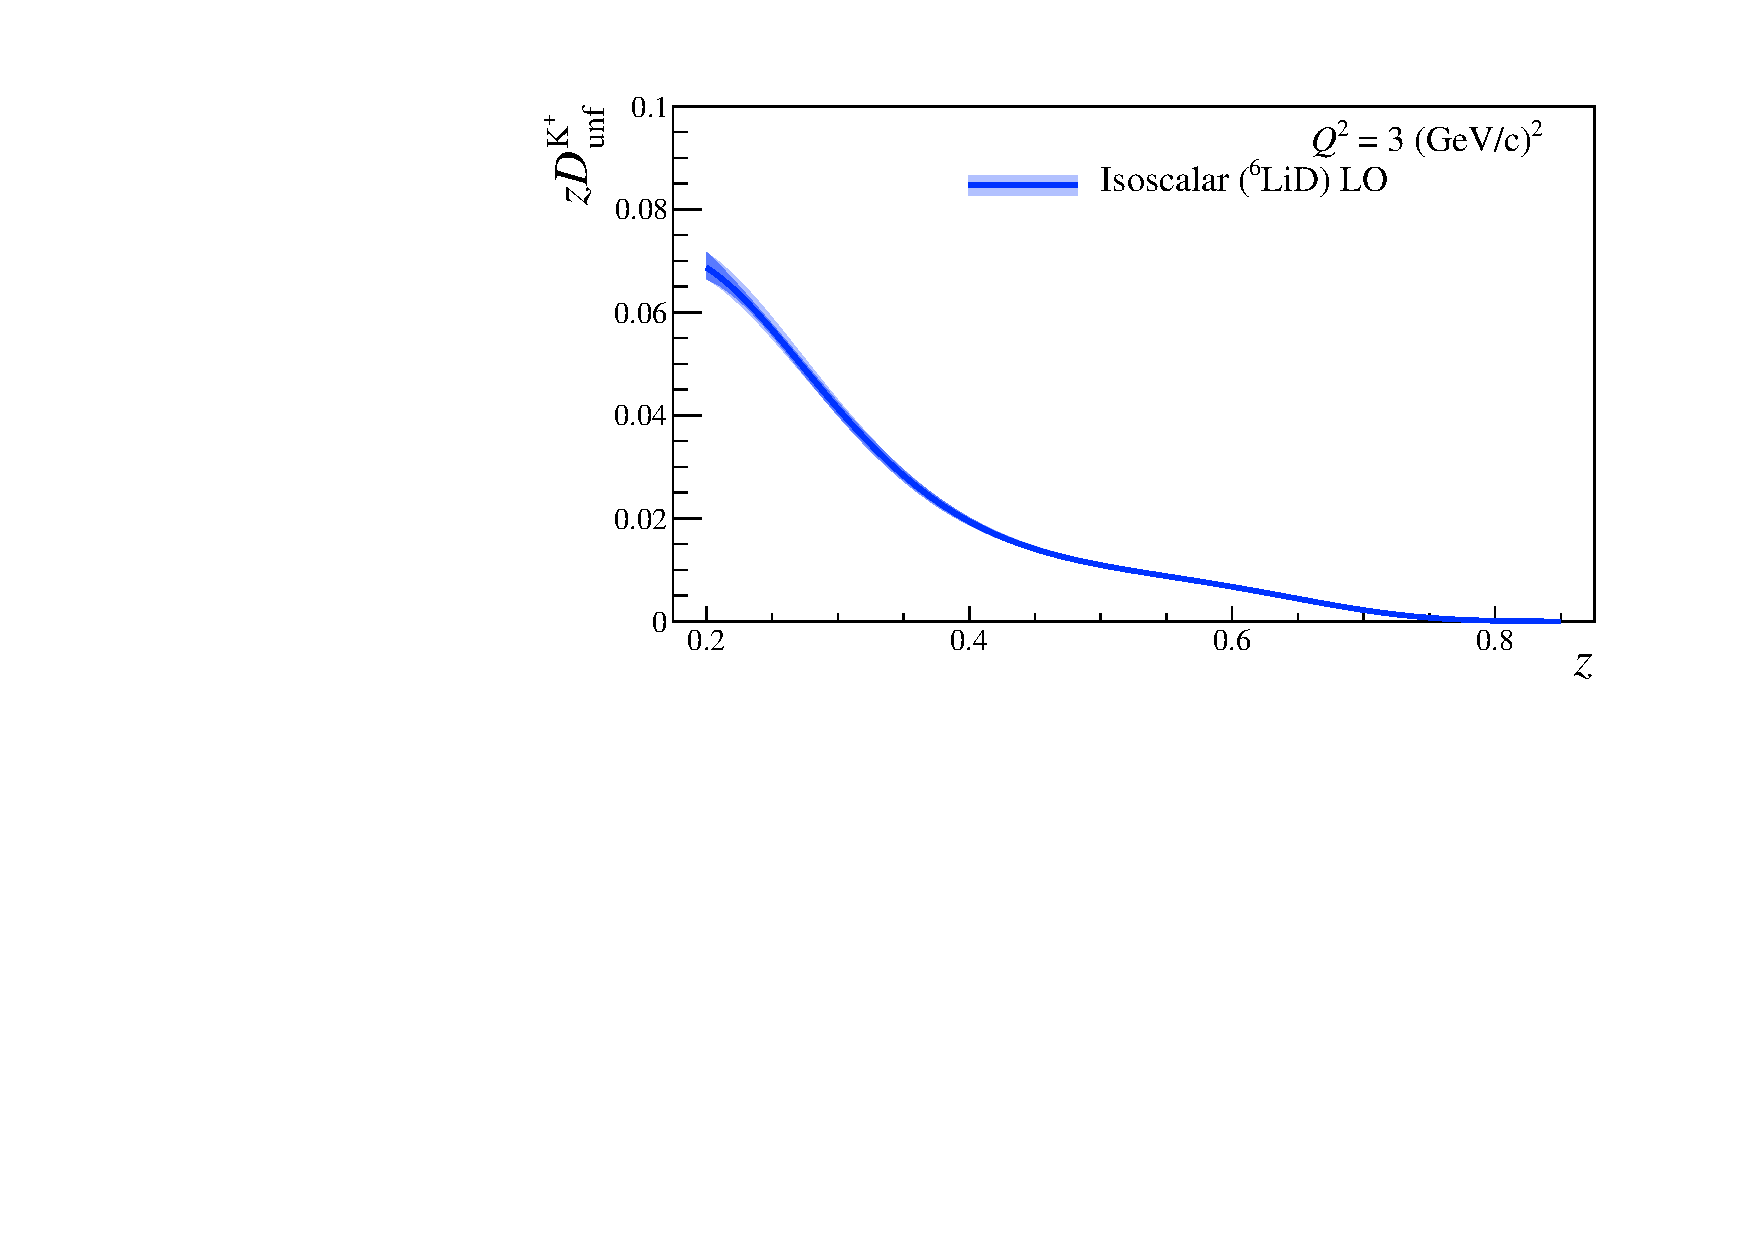
\includegraphics[scale=0.4]{./gfx/dunf.pdf}} \\
  \subfloat[$zD^{K}_{s}$]{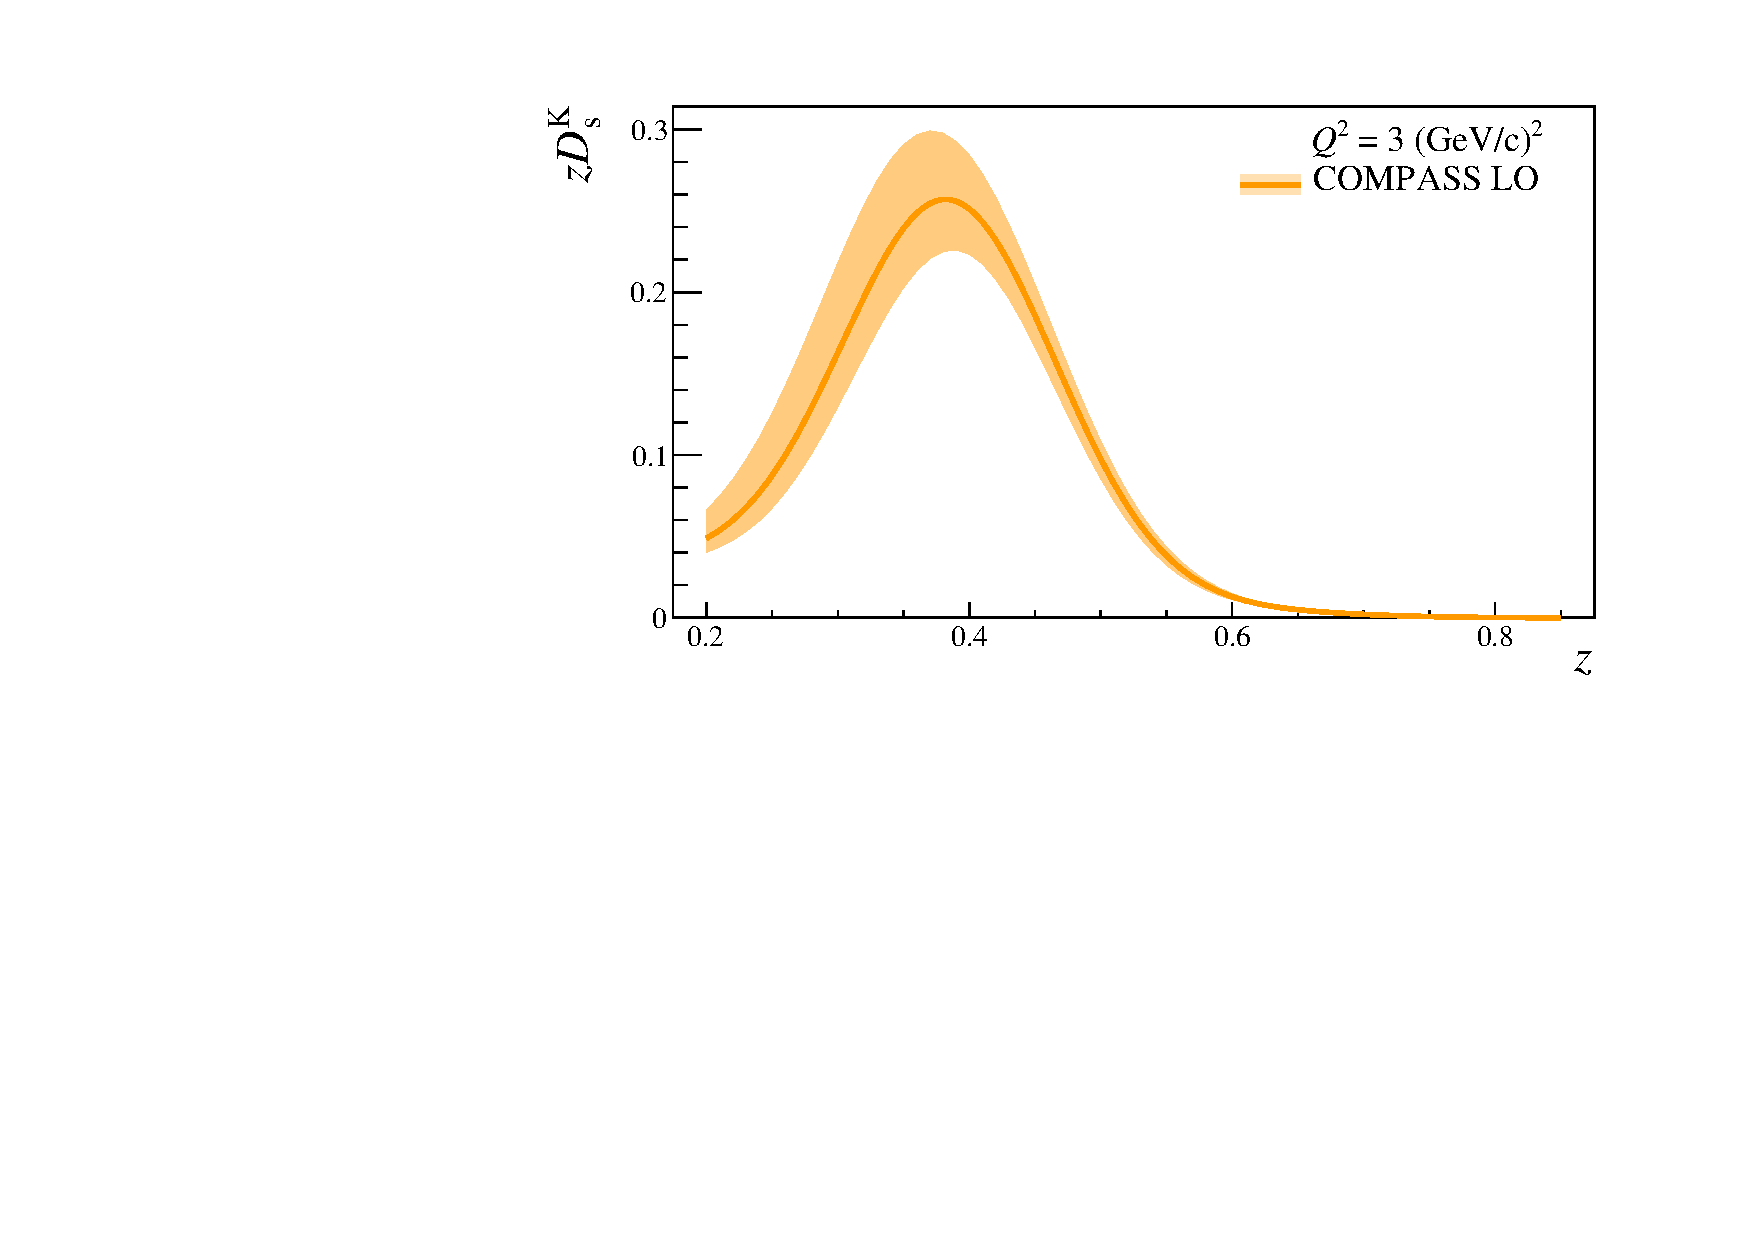
\includegraphics[scale=0.4]{./gfx/dstr.pdf}}
  \subfloat[$zD^{K}_{g}$]{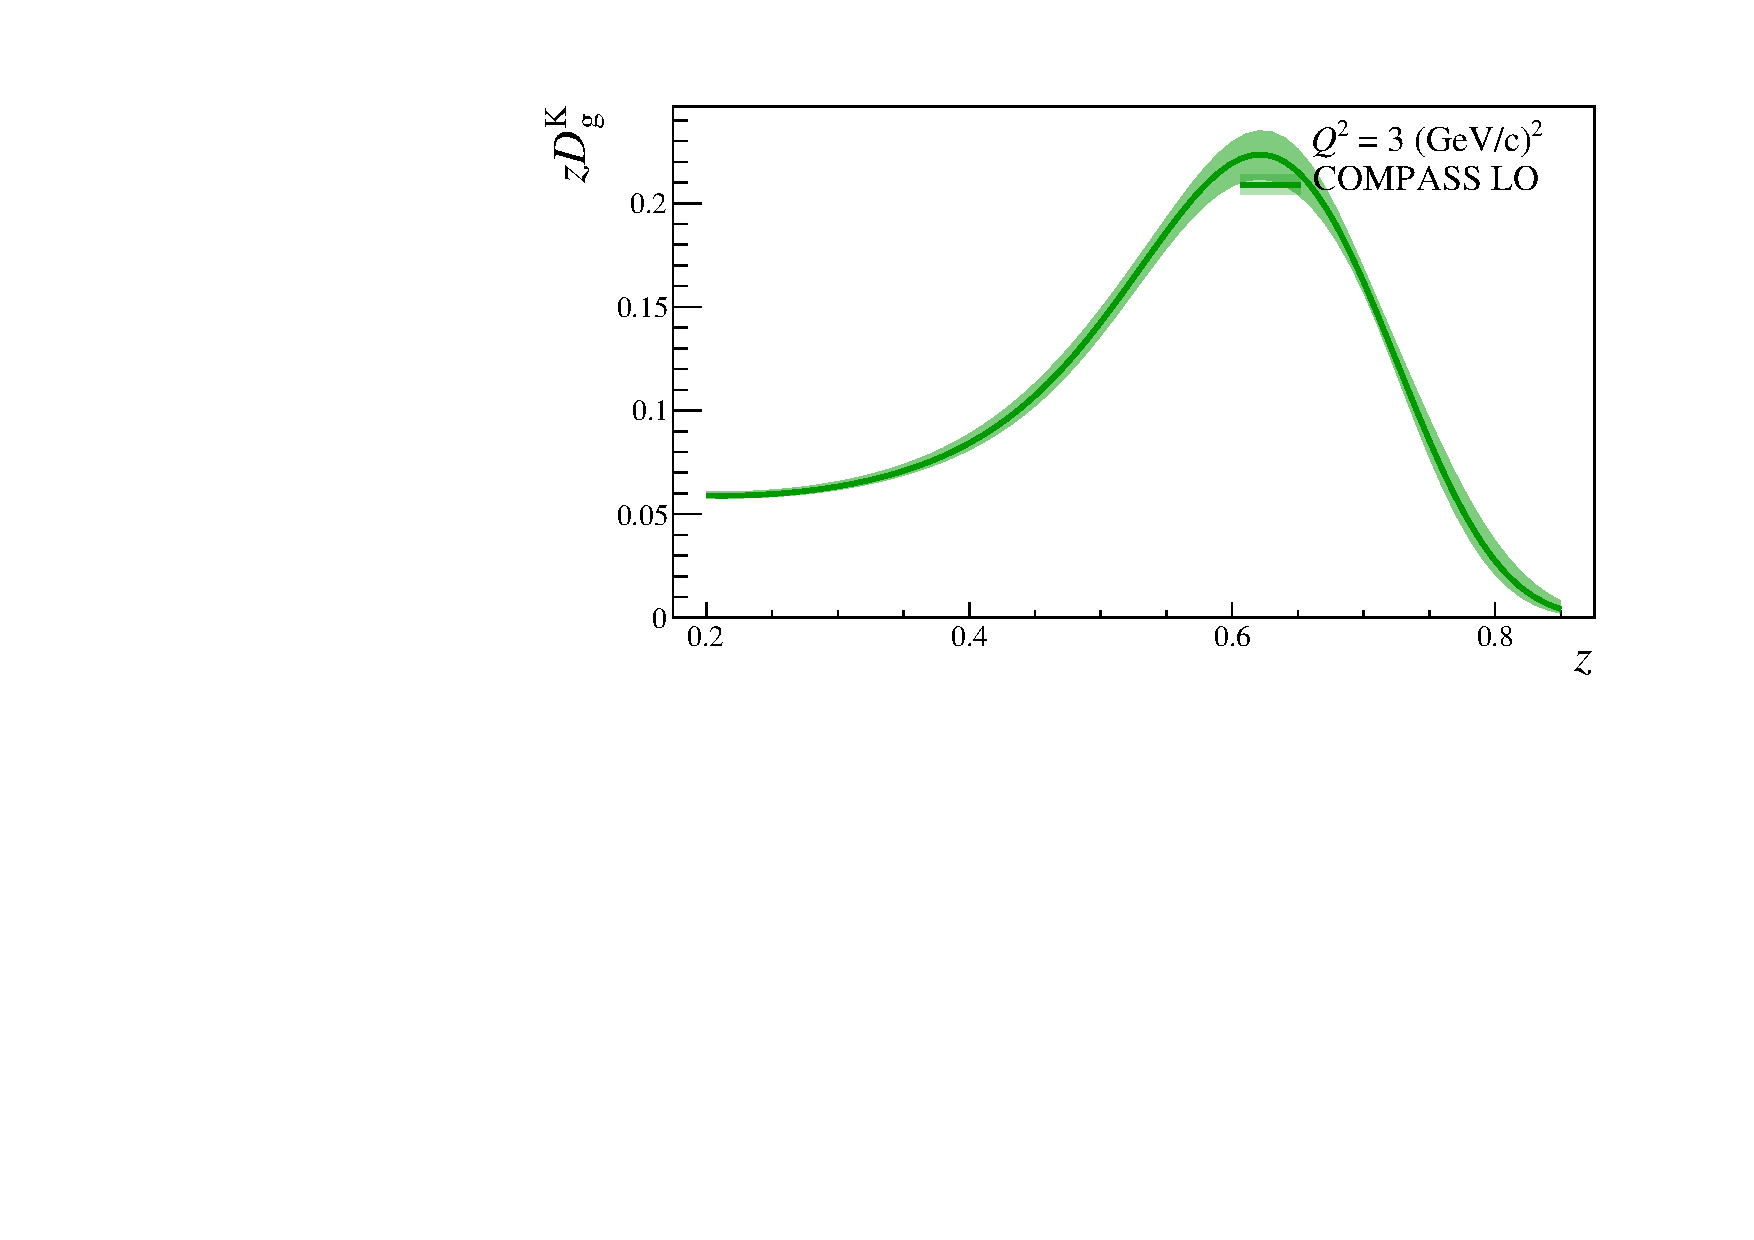
\includegraphics[scale=0.4]{./gfx/dglu.pdf}}
	\caption{The favoured (top left), unfavoured (top right), strange (bottom left) and gluon (bottom right) quark FFs $zD(z)$ into kaons from the COMPASS LO fit. The fit is done based on both the statistical and systematic errors. The green dashed lines are from the same COMPASS LO fit but with COMPASS results for an isoscalar target. The orange dashed line is DSS$07$ LO fit.}
	\label{pic:FApp}
\end{figure}
